\documentclass{beamer}
\usepackage{csc}
\title{Множественное наследование и операторы приведения}

\date{
   \textbf{CS центр}\\
   13 февраля 2018 \\
   Санкт-Петербург
}

\lstset{basicstyle=\fontsize{8pt}{0.92em}\ttfamily,  
        keywordstyle=\fontsize{8pt}{0.92em}\color{MOOCBlue}\bfseries, 
        commentstyle=\fontsize{8pt}{0.92em}\ttfamily\color{MOOCGreen}}

\begin{document}
\begin{frame} 
  \titlepage
\end{frame}

% % % % % % % % % % % % % % % % % % % % % % % % % % % % % % % % %
\begin{frame}[fragile]{Множественное наследование}
    \emph{Множественное наследование (multiple inheritance)}~--- возможность
    наследовать сразу несколько классов.
\medskip
    \begin{lstlisting}
struct Unit {
    Unit(unitid id, int hp): id_(id), hp_(hp) {}
    virtual unitid id() const { return id_; }
    virtual int    hp() const { return hp_; }
private:
    unitid id_;
    int	   hp_;
};

struct Elf:    Unit { ... };
struct Archer: Unit { ... };

struct ElfArcher: Elf, Archer {
    unitid id() const { return Elf::id(); }
    int    hp() const { return Elf::hp(); }
};
    \end{lstlisting}
\end{frame}

% % % % % % % % % % % % % % % % % % % % % % % % % % % % % % % % %
\begin{frame}[fragile]{Представление в памяти}
\begin{center}
\begin{tikzpicture}
   \begin{scope}[thick,
       block/.style={rectangle,draw,fill=cyan!20,minimum size=6mm,minimum width=1.3cm},
	   comp/.style={rectangle,draw,fill=orange!40, minimum size=6mm,minimum width=1.3cm}]
   \node [block] (re)	              				{ElfArcher};
   \node [comp]	 (st)	[above=of re,xshift=+1cm]	{Archer} edge [<-] (re);
   \node [comp]	 (em)	[above=of re,xshift=-1cm]	{Elf}  edge [<-] (re);
   \node [comp]	 (p1)	[above=of st]	            {Unit}   edge [<-] (st);
   \node [comp]	 (p2)	[above=of em]	            {Unit}   edge [<-] (em);
   \end{scope}
\end{tikzpicture}\hfill
\begin{tikzpicture}
\begin{scope}[start chain=1 going right,node distance=-0.15mm,yshift=-3cm]
    \tikzstyle{every path}=[thick]
    \tikzstyle{tmtape}=[draw,minimum height=6mm,fill=orange!40,minimum width=1.3cm]
    \node [on chain=1,tmtape] (p1) {Unit};
    \node [on chain=1,tmtape] (st) {Elf};
    \node [on chain=1,tmtape] (p2) {Unit};
    \node [on chain=1,tmtape] (em) {Archer};
    \node [on chain=1,tmtape,fill=cyan!20] (ea) {ElfArcher};
    \node [below=of p1, yshift=-1cm] (s1) {Elf}    edge [->] (p1.south west);
    \node [below=of s1] {ElfArcher};

    \node [below=of p2, yshift=-1cm] {Archer}    edge [->] (p2.south west);
\end{scope}
\end{tikzpicture}
\end{center}

{\bf Важно:} указатели при приведении могут смещаться.

\end{frame}


% % % % % % % % % % % % % % % % % % % % % % % % % % % % % % % % %
\begin{frame}[fragile]{Создание и удаление объекта}
\begin{center}
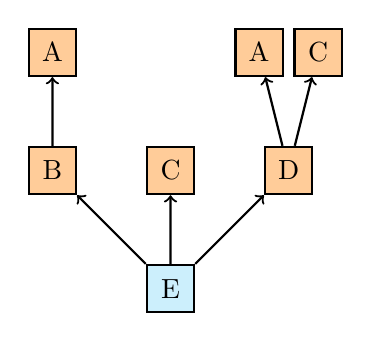
\begin{tikzpicture}[->,thick,
       block/.style={rectangle,draw,fill=cyan!20,minimum size=6mm},
	   comp/.style={rectangle,draw,fill=orange!40, minimum size=6mm},
	   level/.style={sibling distance = 1.5cm/#1, level distance = -1.5cm}]
   \node [block] (a1) {E} 
       child {node [comp] {B}
               child {node [comp] {A}}} 
       child {node [comp] {C}} 
       child {node [comp] {D} 
               child {node [comp] {A}}
               child {node [comp] {C}}};
\end{tikzpicture}
\end{center}


Порядок вызова конструкторов: \texttt{A, B, C, A, C, D, E}.

Деструкторы вызываются в обратном порядке.

Проблемы:
\begin{enumerate}
    \item Дублирование \texttt{A} и \texttt{C}.
    \item Недоступность первого \texttt{C}.
\end{enumerate}

\end{frame}

% % % % % % % % % % % % % % % % % % % % % % % % % % % % % % % % %
\begin{frame}[fragile]{Виртуальное наследование}

\begin{center}
\begin{tikzpicture}[thick,
		block/.style={rectangle,draw,fill=cyan!20,minimum size=6mm,minimum width=1.5cm},
		comp/.style={rectangle,draw,fill=orange!40, minimum size=6mm,minimum width=1.5cm}]
   \node [block] (so)					{Song};
   \node [comp]	 (ly)	[above=of re,xshift=-1cm]	{Lyrics}        edge [<-] (so);
   \node [comp]	 (mu)	[above=of re,xshift=+1cm]	{Music}         edge [<-] (so);
   \node [comp]	 (aw1)	[above=of ly]	            {ArtWork}       edge [<-] (ly);
   \node [comp]	 (aw2)	[above=of mu]	            {ArtWork}       edge [<-] (mu);
\end{tikzpicture}\hspace{2cm}
\begin{tikzpicture}[thick,
		block/.style={rectangle,draw,fill=cyan!20,minimum size=6mm,minimum width=1.5cm},
		comp/.style={rectangle,draw,fill=orange!40, minimum size=6mm,minimum width=1.5cm}]
   \node [block] (so)					            {ElfArcher};
   \node [comp]	 (ly)	[above=of re,xshift=-1cm]	{Elf}        edge [<-] (so);
   \node [comp]	 (mu)	[above=of re,xshift=+1cm]	{Archer}       edge [<-] (so);
   \node<1> [comp]	 (aw1)	[above=of ly,xshift=+1cm]   {Unit}  
        edge [<-] node [color=black,xshift= 6mm] {} (mu)
        edge [<-] node [color=black,xshift=-6mm] {} (ly);
   \node<2> [comp]	 (aw1)	[above=of ly,xshift=+1cm]   {Unit}  
           edge [<-,color=red] node [color=black,xshift= 6mm] {\color{MOOCBlue}{virtual}} (mu)
           edge [<-,color=red] node [color=black,xshift=-6mm] {\color{MOOCBlue}{virtual}} (ly);
\end{tikzpicture}
\end{center}
\pause

    \begin{lstlisting}
struct Unit {};
struct Elf:  virtual Unit {};
struct Archer: virtual Unit {};
struct ElfArcher: Elf, Archer {};
    \end{lstlisting}
\end{frame}

% % % % % % % % % % % % % % % % % % % % % % % % % % % % % % % % %
\begin{frame}[fragile]{Как устроено расположение в памяти?}{}
\vspace{4pt}
\parbox{4cm}{
\begin{tikzpicture}[thick,
		block/.style={rectangle,draw,fill=cyan!20,minimum size=6mm,minimum width=1.5cm},
		comp/.style={rectangle,draw,fill=orange!40, minimum size=6mm,minimum width=1.5cm}]
   \node [block] (so)					            {ElfArcher};
   \node [comp]	 (ly)	[above=of re,xshift=-1cm]	{Elf}        edge [<-] (so);
   \node [comp]	 (mu)	[above=of re,xshift=+1cm]	{Archer}       edge [<-] (so);
   \node [comp]	 (aw1)	[above=of ly,xshift=+1cm]   {Unit}  
        edge [<-,color=red] node [color=black,xshift= 6mm] {\color{MOOCBlue}{virtual}} (mu)
        edge [<-,color=red] node [color=black,xshift=-6mm] {\color{MOOCBlue}{virtual}} (ly);
\end{tikzpicture}}\parbox{6cm}{
\begin{tikzpicture}
    \tikzstyle{every path}=[thick]
    \tikzstyle{tmtape}=[draw,minimum height=6mm, minimum width=1.5cm]
\begin{scope}[start chain=1 going right,node distance=-0.15mm]
    \node [on chain=1,tmtape,draw=none, minimum width=25mm] {Elf};
    \node [on chain=1,tmtape] {Unit};
    \node [on chain=1,tmtape] {Elf};
\end{scope}
\begin{scope}[start chain=1 going right,node distance=-0.15mm,yshift=-1cm]
    \node [on chain=1,tmtape,draw=none, minimum width=25mm] {Archer};
    \node [on chain=1,tmtape] {Unit};
    \node [on chain=1,tmtape] {Archer};
\end{scope}
\begin{scope}[start chain=1 going right,node distance=-0.15mm,yshift=-2cm]
    \node [on chain=1,tmtape,draw=none, minimum width=25mm] {ElfArcher?};
    \node [on chain=1,tmtape] {Unit};
    \node [on chain=1,tmtape] {Elf};
    \node [on chain=1,tmtape] {Archer};
\end{scope}
\begin{scope}[start chain=1 going right,node distance=-0.15mm,yshift=-3cm]
    \node [on chain=1,tmtape,draw=none, minimum width=25mm] {ElfArcher?};
    \node [on chain=1,tmtape] {Elf};
    \node [on chain=1,tmtape] {Unit};
    \node [on chain=1,tmtape] {Archer};
\end{scope}
\end{tikzpicture}}
\vskip5mm\pause

\parbox{4cm}{
На самом деле.}\parbox{6cm}{
\begin{tikzpicture}
    \tikzstyle{every path}=[thick]
    \tikzstyle{tmtape}=[draw,minimum height=6mm, minimum width=1.5cm]
\begin{scope}[start chain=1 going right,node distance=-0.15mm]
    \node [on chain=1,tmtape,draw=none, minimum width=25mm] {Elf};
    \node [on chain=1,tmtape] {Elf};
    \node [on chain=1,tmtape] {Unit};
\end{scope}
\begin{scope}[start chain=1 going right,node distance=-0.15mm,yshift=-1cm]
    \node [on chain=1,tmtape,draw=none, minimum width=25mm] {Archer};
    \node [on chain=1,tmtape] {Archer};
    \node [on chain=1,tmtape] {Unit};
\end{scope}
\begin{scope}[start chain=1 going right,node distance=-0.15mm,yshift=-2cm]
    \tikzstyle{every path}=[thick]
    \tikzstyle{tmtape}=[draw,minimum height=6mm, minimum width=1.5cm]
    \node [on chain=1,tmtape,draw=none, minimum width=25mm] {ElfArcher};
    \node [on chain=1,tmtape] {Elf};
    \node [on chain=1,tmtape] {Archer};
    \node [on chain=1,tmtape] {Unit};
\end{scope}
\end{tikzpicture}}
\end{frame}

% % % % % % % % % % % % % % % % % % % % % % % % % % % % % % % % %
\begin{frame}[fragile]{Доступ через таблицу виртуальных методов}
    \begin{lstlisting}
struct Unit { 
    unitid id;
};
struct Elf  : virtual Unit { };
struct Archer : virtual Unit { };
struct ElfArcher : Elf, Archer { };
    \end{lstlisting}
    \pause
Рассмотрим такой код:
    \begin{lstlisting}
    Elf * e = (rand() % 2)? new Elf() : new ElfArcher();
    unitid id = e->id; // (*)
    \end{lstlisting}
    \pause
Строка \texttt{(*)} будет преобразована в строку
    \begin{lstlisting}
    unitid id = e->__getUnitPtr__()->id;
    \end{lstlisting}
где \texttt{\_\_getUnitPtr\_\_()}~— это служебный виртуальный метод.
\end{frame}


% % % % % % % % % % % % % % % % % % % % % % % % % % % % % % % % %
\begin{frame}[fragile]{Кто вызывает конструктор базового класса?}
\begin{minipage}{.6\textwidth}
    \begin{lstlisting}
struct Unit { 
    Unit(unitid id, int health_points); 
};
struct Elf: virtual Unit {
    explicit Elf(unitid id) 
        : Unit(id, 100) {}
};
struct Archer: virtual Unit {
    explicit Archer(unitid id) 
        : Unit(id, 120) {}
};
struct ElfArcher: Elf, Archer {
    explicit ElfArcher(unitid id) 
        : Unit(id, 150)
        , Elf(id)
        , Archer(id) {}
};
    \end{lstlisting}
\end{minipage}\hspace{10mm}
\begin{minipage}{.25\textwidth}
\begin{tikzpicture}[thick,
		block/.style={rectangle,draw,fill=cyan!20,minimum size=6mm,minimum width=1.5cm},
		comp/.style={rectangle,draw,fill=orange!40, minimum size=6mm,minimum width=1.5cm}]
   \node [block] (so)					            {ElfArcher};
   \node [comp]	 (ly)	[above=of re,xshift=-1cm]	{Elf}        edge [<-] (so);
   \node [comp]	 (mu)	[above=of re,xshift=+1cm]	{Archer}       edge [<-] (so);
   \node [comp]	 (aw1)	[above=of ly,xshift=+1cm]   {Unit}  
           edge [<-,color=red] node [color=black,xshift= 6mm] {\color{MOOCBlue}{virtual}} (mu)
           edge [<-,color=red] node [color=black,xshift=-6mm] {\color{MOOCBlue}{virtual}} (ly);
\end{tikzpicture}
\end{minipage}

\end{frame}

% % % % % % % % % % % % % % % % % % % % % % % % % % % % % % % % %
\begin{frame}[fragile]{Заключение}
    \begin{itemize}
        \item Не используйте множественное наследование для наследования
            реализации.
        
        \pitem Используйте концепцию интерфейсов (классы без реализаций и членов данных).

        \pitem Помните о неприятностях, связанных с множественным наследованием.

        \pitem Хорошо подумайте перед тем, как использовать виртуальное
            наследование.

        \pitem Помните о неприятностях, связанных с виртуальным наследованием.
    \end{itemize}
\end{frame}

%%%%%%%%%%%%%%%%%%%%%%%%%%%%%%%%%%%%%%%%%%%%%%%%%%%%%%%%%%%%%%%%
\begin{frame}[fragile]{Преобразование в стиле \langc}{}
В \langc этот оператор преобразует встроенные типы и указатели.
\begin{lstlisting}
int a = 2;
int b = 3;
    
// int $\to$ double
double size = ((double)a) / b * 100; 

// double $\to$ int
void * data = malloc(sizeof(double) * int(size));

// void * $\to$ double *
double * array = (double *)data; 

// double * $\to$ char *
char * bytes = (char *)array;
\end{lstlisting}
\end{frame}

\begin{frame}[fragile]{Преобразования в \langcpp: \code{static\_cast}}
    Служит для преобразований связанных типов:
    \begin{itemize}
        \pitem Стандартные преобразования.
        \begin{itemize}
\item Преобразования числовых типов.
\begin{lstlisting}
double s = static_cast<double>(2) / 3 * 100; 
s = static_cast<int>(d);
\end{lstlisting}
\item Указатель/ссылка на производный класс в указатель/ссылку на базовый класс.
\item \texttt{T*} в \code{void}\texttt{*}.
        \end{itemize}
        \pitem Явное (пользовательское) приведение типа:
\begin{lstlisting}
Person p = static_cast<Person>("Ivan");
\end{lstlisting}
        \pitem Обратные варианты стандартных преобразований:
            \begin{itemize}
                %\item целочисленные типы в перечисляемые,
                \item Указатель/ссылка на базовый класс в указатель/ссылку на производный класс (преобразование вниз, downcast),
                %\item {\tt T Base::*} в {\tt T Derived::*},
                \item \code{void}\texttt{*} в любой {\tt T*}.                          
            \end{itemize}
        \pitem Преобразование к \code{void}.
    \end{itemize}
\end{frame}

\begin{frame}[fragile]{Преобразования в \langcpp: \code{const\_cast}}
    Служит для снятия/добавления константности.\pause
\begin{lstlisting}
    void foo(double const& d) {
        const_cast<double &>(d) = 10;
    } 
\end{lstlisting}
Использование \code{const\_cast}~--- признак плохого дизайна.\\
\medskip\pause
Кроме редких исключений:
\begin{lstlisting}
T & operator[](size_t i) {
    return const_cast<T &>(
           const_cast<Vector const &>(*this)[i]);
}

T const & operator[](size_t i) const {
    assert(i < size_);
    return data_[i];
}
\end{lstlisting}
\end{frame}

\begin{frame}[fragile]{Преобразования в \langcpp: \code{reinterpret\_cast}}{}
    Служит для преобразований указателей и ссылок на несвязанные типы.\pause
    
\begin{lstlisting}
void send(char const * data, size_t length);
char * receive(size_t * length);
\end{lstlisting}\pause
\begin{lstlisting}
double * m = static_cast<double*>(malloc(sizeof(double) * 100)); 
... // инициализация m
char * mc = reinterpret_cast<char *>(m);
send(mc, sizeof(double) * 100);
\end{lstlisting}\pause
\begin{lstlisting}
size_t length = 0;
double * m = reinterpret_cast<double*>(receive(&length));
length = length / sizeof(double);
\end{lstlisting}\pause

Поможет преобразовать указатель в число.
\begin{lstlisting}
size_t ms = reinterpret_cast<size_t>(m);
\end{lstlisting}
\end{frame}

\begin{frame}[fragile]{Границы применимости преобразования в стиле \langc}{}
  \begin{itemize}
    \pitem Преобразования в стиле \langc может заменить любое из рассмотренных преобразований: 
    \begin{itemize}
        \item \code{static\_cast},
        \item \code{reinterpret\_cast},
        \item \code{const\_cast}.
    \end{itemize}

    \pitem Преобразования в стиле \langc можно использовать для
    \begin{itemize}
        \item преобразование встроенных типов,
        \item преобразование указателей на явные типы.
    \end{itemize}

    \pitem Преобразования в стиле \langc не стоит использовать:
    \begin{itemize}
        \item с пользовательскими типами и указателями на них,
        \item в шаблонах.        
    \end{itemize}
  \end{itemize}
\end{frame}

\begin{frame}[fragile]{Когда преобразование в стиле \langc приводит к ошибке}{}
\begin{lstlisting}
// abc.h
struct A { int a; };

struct B {};

struct C : A, B {};
\end{lstlisting}

\pause
\begin{minipage}{.45\textwidth}
\begin{lstlisting}
#include "abc.h"

C * foo(B * b) {
    return (C *)b;
}
\end{lstlisting}

\only<4>{\raggedright 
\small Если в этой точке известны определения классов,\\ то происходит преобразование \code{static\_cast}.}

\end{minipage}\pause\hfill
\begin{minipage}{.51\textwidth}
\begin{lstlisting}
struct A; struct B; struct C;

C * foo(B * b) {
    return (C *)b;
}
\end{lstlisting}
\only<4>{\raggedright 
\small Если известны только\\ объявления, то происходит преобразование \code{reinterpret\_cast}.}
\end{minipage}
\end{frame}

%%%%%%%%%%%%%%%%%%%%%%%%%%%%%%%%%%%%%%%%%%%%%%%%%%%%%%%%%%%%%%%%%
\begin{frame}[fragile]{Run-Time Type Information (RTTI)}
В \langcpp этот механизм состоит из двух компонент:
\begin{enumerate}
    \item оператор \code{typeid} и тип \texttt{std::type\_info},
    \item оператор \code{dynamic\_cast}.
\end{enumerate}
\pause
\begin{block}{Тип {\tt type\_info}}
    \begin{itemize}
        \item Класс, объявленный в \texttt{<typeinfo>}.
        \item Содержит информацию о типе.
        \item Методы: \texttt{==, !=, name, before}.
        \item Нет публичных конструкторов и оператора присваивания.
        \item Можно получить ссылку на \texttt{type\_info}, соответствующий\\ значению или типу, при помощи оператора \code{typeid}.
    \end{itemize}
\end{block}
\end{frame}

\begin{frame}[fragile]{Использование \texttt{typeid} и {\tt type\_info}}
    \begin{lstlisting}
struct Unit { 
    // наличие виртуальных методов необходимо
    virtual ~Unit() { } 
}; 

struct Elf : Unit { };

int main() {
    Elf e;
    Unit & ur = e;
    Unit * up = &e;
    cout << typeid(ur) .name() << endl; // Elf
    cout << typeid(*up).name() << endl; // Elf
    cout << typeid(up) .name() << endl; // Unit *
    cout << typeid(Elf).name() << endl; // Elf
    cout << (typeid(ur) == typeid(Elf)); // 1
}
    \end{lstlisting}
\end{frame}

\begin{frame}[fragile]{Преобразования в \langcpp: {\tt dynamic\_cast}}
    Преобразования с проверкой типа времени выполнения.
    \begin{lstlisting}
Unit * u = (rand() % 2)? new Elf(): new Dwarf();
...
if (Elf * e = dynamic_cast<Elf *>(u))
    ...
else if (Dwarf * d = dynamic_cast<Dwarf *>(u))
    ...        
    \end{lstlisting}
\pause    
Особенности:
    \begin{itemize}
        \item Не заменяется преобразованием в стиле \langc.
        \item Требует наличие виртуальных функций (полиморфность).
    \end{itemize}
\pause
Вопросы:
\begin{itemize}
    \item Почему следует избегать RTTI?
    \item Что возвращает {\tt \code{dynamic\_cast}<\code{void} *>(u)}?
\end{itemize}
\end{frame}

\begin{frame}[fragile]{Пример обхода \texttt{dynamic\_cast}: double dispatch}
\begin{lstlisting}
struct Rectangle; struct Circle;

struct Shape { 
    virtual ~Shape() {} 
    virtual bool intersect( Rectangle * r ) = 0;
    virtual bool intersect( Circle    * c ) = 0;
    virtual bool intersect( Shape     * s ) = 0;
};

struct Circle : Shape {
    bool intersect( Rectangle * r ) { ... }
    bool intersect( Circle    * c ) { ... }
    bool intersect( Shape     * s ) { 
        return s->intersect(this); 
    }
};
bool intersect(Shape * a, Shape * b) { 
    return a->intersect(b); 
}
\end{lstlisting}
\end{frame}

%%%%%%%%%%%%%%%%%%%%%%%%%%%%%%%%%%%%%%%%%%%%%%%%%%%%%%%%%%%%%%%%%%%

\end{document}


